\documentclass[journal, a4paper]{IEEEtran}

% some very useful LaTeX packages include:

%\usepackage{cite}      % Written by Donald Arseneau
                        % V1.6 and later of IEEEtran pre-defines the format
                        % of the cite.sty package \cite{} output to follow
                        % that of IEEE. Loading the cite package will
                        % result in citation numbers being automatically
                        % sorted and properly "ranged". i.e.,
                        % [1], [9], [2], [7], [5], [6]
                        % (without using cite.sty)
                        % will become:
                        % [1], [2], [5]--[7], [9] (using cite.sty)
                        % cite.sty's \cite will automatically add leading
                        % space, if needed. Use cite.sty's noadjust option
                        % (cite.sty V3.8 and later) if you want to turn this
                        % off. cite.sty is already installed on most LaTeX
                        % systems. The latest version can be obtained at:
                        % http://www.ctan.org/tex-archive/macros/latex/contrib/supported/cite/

\usepackage{graphicx}   % Written by David Carlisle and Sebastian Rahtz
                        % Required if you want graphics, photos, etc.
                        % graphicx.sty is already installed on most LaTeX
                        % systems. The latest version and documentation can
                        % be obtained at:
                        % http://www.ctan.org/tex-archive/macros/latex/required/graphics/
                        % Another good source of documentation is "Using
                        % Imported Graphics in LaTeX2e" by Keith Reckdahl
                        % which can be found as esplatex.ps and epslatex.pdf
                        % at: http://www.ctan.org/tex-archive/info/

%\usepackage{psfrag}    % Written by Craig Barratt, Michael C. Grant,
                        % and David Carlisle
                        % This package allows you to substitute LaTeX
                        % commands for text in imported EPS graphic files.
                        % In this way, LaTeX symbols can be placed into
                        % graphics that have been generated by other
                        % applications. You must use latex->dvips->ps2pdf
                        % workflow (not direct pdf output from pdflatex) if
                        % you wish to use this capability because it works
                        % via some PostScript tricks. Alternatively, the
                        % graphics could be processed as separate files via
                        % psfrag and dvips, then converted to PDF for
                        % inclusion in the main file which uses pdflatex.
                        % Docs are in "The PSfrag System" by Michael C. Grant
                        % and David Carlisle. There is also some information
                        % about using psfrag in "Using Imported Graphics in
                        % LaTeX2e" by Keith Reckdahl which documents the
                        % graphicx package (see above). The psfrag package
                        % and documentation can be obtained at:
                        % http://www.ctan.org/tex-archive/macros/latex/contrib/supported/psfrag/

%\usepackage{subfigure} % Written by Steven Douglas Cochran
                        % This package makes it easy to put subfigures
                        % in your figures. i.e., "figure 1a and 1b"
                        % Docs are in "Using Imported Graphics in LaTeX2e"
                        % by Keith Reckdahl which also documents the graphicx
                        % package (see above). subfigure.sty is already
                        % installed on most LaTeX systems. The latest version
                        % and documentation can be obtained at:
                        % http://www.ctan.org/tex-archive/macros/latex/contrib/supported/subfigure/

\usepackage{url}        % Written by Donald Arseneau
                        % Provides better support for handling and breaking
                        % URLs. url.sty is already installed on most LaTeX
                        % systems. The latest version can be obtained at:
                        % http://www.ctan.org/tex-archive/macros/latex/contrib/other/misc/
                        % Read the url.sty source comments for usage information.

%\usepackage{stfloats}  % Written by Sigitas Tolusis
                        % Gives LaTeX2e the ability to do double column
                        % floats at the bottom of the page as well as the top.
                        % (e.g., "\begin{figure*}[!b]" is not normally
                        % possible in LaTeX2e). This is an invasive package
                        % which rewrites many portions of the LaTeX2e output
                        % routines. It may not work with other packages that
                        % modify the LaTeX2e output routine and/or with other
                        % versions of LaTeX. The latest version and
                        % documentation can be obtained at:
                        % http://www.ctan.org/tex-archive/macros/latex/contrib/supported/sttools/
                        % Documentation is contained in the stfloats.sty
                        % comments as well as in the presfull.pdf file.
                        % Do not use the stfloats baselinefloat ability as
                        % IEEE does not allow \baselineskip to stretch.
                        % Authors submitting work to the IEEE should note
                        % that IEEE rarely uses double column equations and
                        % that authors should try to avoid such use.
                        % Do not be tempted to use the cuted.sty or
                        % midfloat.sty package (by the same author) as IEEE
                        % does not format its papers in such ways.

\usepackage{amsmath}    % From the American Mathematical Society
                        % A popular package that provides many helpful commands
                        % for dealing with mathematics. Note that the AMSmath
                        % package sets \interdisplaylinepenalty to 10000 thus
                        % preventing page breaks from occurring within multiline
                        % equations. Use:
%\interdisplaylinepenalty=2500
                        % after loading amsmath to restore such page breaks
                        % as IEEEtran.cls normally does. amsmath.sty is already
                        % installed on most LaTeX systems. The latest version
                        % and documentation can be obtained at:
                        % http://www.ctan.org/tex-archive/macros/latex/required/amslatex/math/



% Other popular packages for formatting tables and equations include:

%\usepackage{array}
% Frank Mittelbach's and David Carlisle's array.sty which improves the
% LaTeX2e array and tabular environments to provide better appearances and
% additional user controls. array.sty is already installed on most systems.
% The latest version and documentation can be obtained at:
% http://www.ctan.org/tex-archive/macros/latex/required/tools/

% V1.6 of IEEEtran contains the IEEEeqnarray family of commands that can
% be used to generate multiline equations as well as matrices, tables, etc.

% Also of notable interest:
% Scott Pakin's eqparbox package for creating (automatically sized) equal
% width boxes. Available:
% http://www.ctan.org/tex-archive/macros/latex/contrib/supported/eqparbox/

% *** Do not adjust lengths that control margins, column widths, etc. ***
% *** Do not use packages that alter fonts (such as pslatex).         ***
% There should be no need to do such things with IEEEtran.cls V1.6 and later.


% Your document starts here!
\begin{document}

% Define document title and author
    \title{Midterm Report: Predictive Analysis of City Crime Hotspots}
    \author{Sahil Deshpande, Vinit Kumar \\ $\{sahilsd, vinitn\}@bu.edu$}
    \maketitle

% Write abstract here
\begin{abstract}
    With increased digitization of data around the world, various type of data is now easily available. This includes criminal reports for most of the major cities in the US. In order to constructively use this data and the available data mining tools in Python, we are trying to analyze crime hotspots and predict next most likely crime location. 
\end{abstract}

% Each section begins with a \section{title} command
\section{Introduction}
   Crimes have become a common part of city life that seriously affect quality of life and economic growth of a society. Universal organizations are spending a lot of resources trying to identify safest and most dangerous cities to help local authorities manage their workforce. As more and more people shift to the city, this concentrated population makes it important to find safer places. Using the open-source data from official websites and some of the basic data mining approaches, we are attempting to help this process [1].  

   From past analysis of various cities and their neighbourhoods, it has been shown that certain parts of the city are more prone to criminal activities than others making them a criminal hotspot. Even though there doesn't seem to be an intuitive pattern for criminals, they tend to favor certain areas that makes it possible to predict such malicious activities. Using the information about past activities, law enforcements can effectively serve their duties. 

   To achieve this predictive analysis, we have looked at various datasets available for free on the Internet[2-3]. After some research on which cities have most relevant and most updated data, we have decided to work with Boston, Los Angeles and Raleigh. The first part of this project is to get the data in a specified format (in this case json) and parse it to extract meaningful information. Using these parsed data structures, we are interested in finding the most relevant crime types such as assault, robbery, hit and run, to name a few. We select the types that affect a particular area the most using regression techniques[4]. After trimming the dataset, we have applied k-means clustering to plot these various types of activities using GMplot[5]. We now plan to use classification methods in order to predict most vulnerable parts of the city. Later sections describe the results we've seen so far.
% Main Part
    \begin{figure}[!hbt]
        % Center the figure.
        \begin{center}
        % Include the eps file, scale it such that it's width equals the column width. You can also put width=8cm for example...
        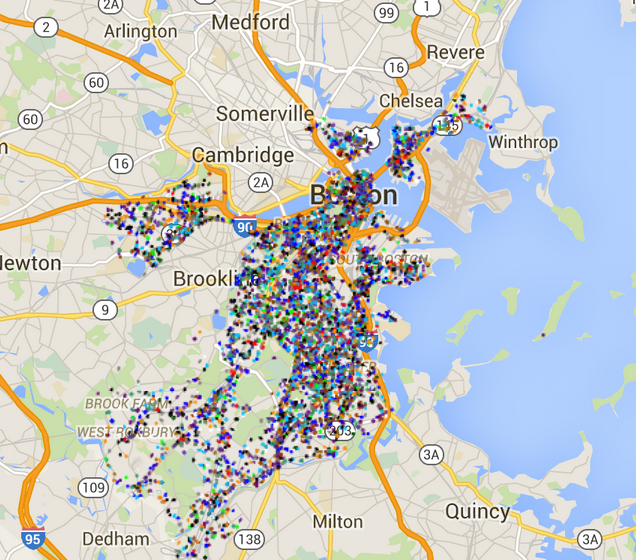
\includegraphics[width=\columnwidth]{fig1.png}
        % Create a subtitle for the figure.
        \caption{Overall crime distribution across Boston shows concentrated crime data.}
        % Define the label of the figure. It's good to use 'fig:title', so you know that the label belongs to a figure.
        \label{fig:tf_plot}
        \end{center}
    \end{figure}

    \begin{figure}[!hbt]
        % Center the figure.
        \begin{center}
        % Include the eps file, scale it such that it's width equals the column width. You can also put width=8cm for example...
        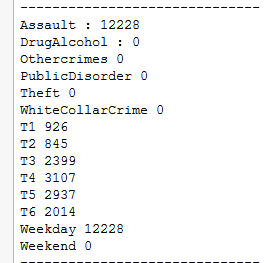
\includegraphics[width=\columnwidth]{fig2.png}
        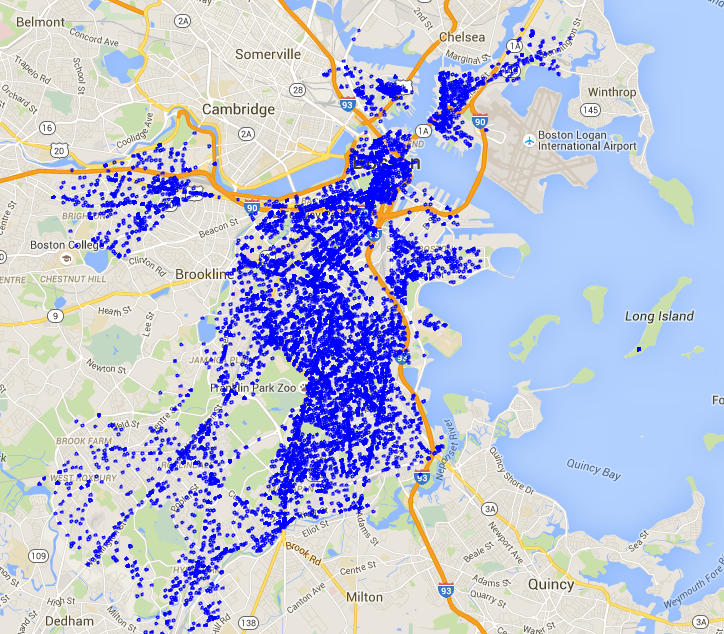
\includegraphics[width=\columnwidth]{fig3.png}
        % Create a subtitle for the figure.
        \caption{Cluster showing only Assault crimes and only on weekdays.}
        % Define the label of the figure. It's good to use 'fig:title', so you know that the label belongs to a figure.
        \label{fig:tf_plot}
        \end{center}
    \end{figure}

    \begin{figure}[!hbt]
        % Center the figure.
        \begin{center}
        % Include the eps file, scale it such that it's width equals the column width. You can also put width=8cm for example...
        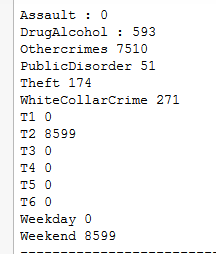
\includegraphics[width=\columnwidth]{fig4.png}
        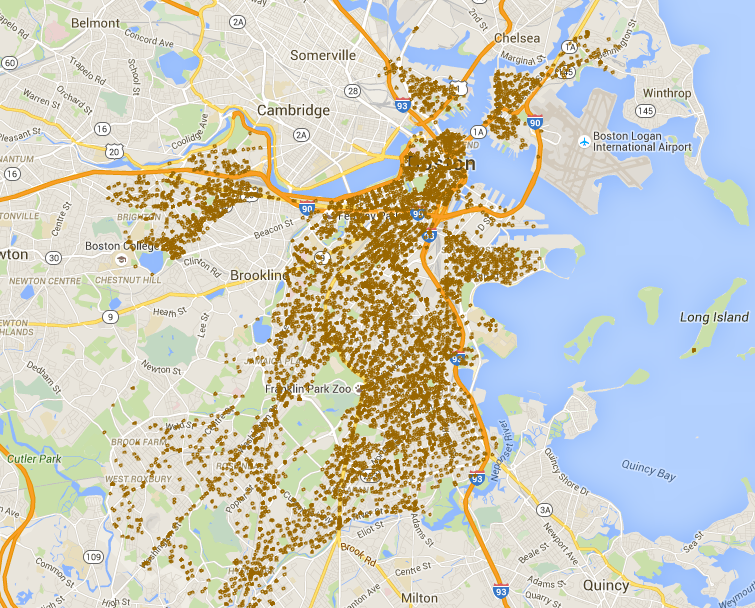
\includegraphics[width=\columnwidth]{fig5.png}
        % Create a subtitle for the figure.
        \caption{Cluster showing only crimes only on weekends.}
        % Define the label of the figure. It's good to use 'fig:title', so you know that the label belongs to a figure.
        \label{fig:tf_plot}
        \end{center}
    \end{figure}

\section{Technique}
    First we searched on the Internet for reliable data sources for criminal activities in major cities in US. After going through large number of datafiles, we decided to work with data from [3]. After getting the data in json format, we parsed it to get attributes such as crime location, latitude and longitude, time of crime, day of the week, type of the crime. Since these attributes help us distinguish between most of the important crime activities, we plan to use these attributes for further analysis. 

    While parsing the data, we have also divided the timestamps into six categories and day of the week as weekday or weekend. This further enables more meaningful clustering because coarse datasets are clustered more effectively.

    In order to reduce this large data, we are now planning to use linear and logistic regression to find which crime types affect an area the most. Here we can calculate an average score for one area based on crime types (as we did in homework) and get top five coefficients that will denote the most common crime types. As we know, more data helps in better analysis and prediction we wanted to minimize this data reduction and thought this technique would be most effective.

    For now, we have skipped the regression step and directly went on to categorize the data in types like assault, robbery, disturbance, white collar crime and others. But this can be easily replaced with the types we get from regression results so we are first focusing on analysis part. Using these categories, we have applied K-means clustering from Python sklearn. The clustering results are explained in the next section. We have normalized the latitude and longitude during clustering so that they don't add any extra weight. While plotting the clusters on the map, we have used the original latitudes and longitudes to give correct crime hotspots.

    So this has given us a basic idea of malicious activities and their patterns in Boston. We can easily identify which areas show more assaults or weekend crime. This example already starts to unfold the advantages after seeing which areas are relatively safer and which would need more attention of local law enforcement. Using this clustered data, we are now exploring classifier methods in python which were discussed in the class. Right now we have come up with two approaches on how we can predict a crime but this part needs more work. First approach is to directly use latitude/longitude for predicting most likely crime activity but this has very fine granularity which makes it less favorable. On the other hand, we are planning to utilize area codes in the data set. This divide the city in certain code like A4, G1, etc. We can use these and one of the six timestamps and try to get a tuple similar to, <type of crime, area code, time category, day category>. We think this will be more clear after the Amazon prediction assignment. We plan to revisit this once more.
    
\section{Experiments}
    For initial phase of analysis, we tried to focus on dataset for Boston. The initial code is available in a private repository at [6]. This stage consists of parsing data, reducing data and clustering. After reviewing the dataset, we managed to select few crime types for initial experiments. Using these types along with time of day, day of the week and latitude/longitude pair we executed K-means clustering and plotted it using GMplot.  

    % This is how you define a table: the [!hbt] means that LaTeX is forced (by the !) to place the table exactly here (by h), or if that doesnt work because of a pagebreak or so, it tries to place the table to the bottom of the page (by b) or the top (by t).
    %\begin{table}[!hbt]
        % Center the table
        %\begin{center}
        % Title of the table
        %\caption{Simulation Parameters}
        %\label{tab:simParameters}
        % Table itself: here we have two columns which are centered and have lines to the left, right and in the middle: |c|c|
        %\begin{tabular}{|c|c|}
            % To create a horizontal line, type \hline
            %\hline
            % To end a column type &
            % For a linebreak type \\
            %Information message length & $k=16000$ bit \\
            %\hline
            %Radio segment size & $b=160$ bit \\
            %\hline
            %Rate of component codes & $R_{cc}=1/3$\\
            %\hline
            %Polynomial of component encoders & $[1 , 33/37 , 25/37]_8$\\
            %\hline
        %\end{tabular}
        %\end{center}
    %\end{table}

    % If you have questions about how to write mathematical formulas in LaTeX, please read a LaTeX book or the 'Not So Short Introduction to LaTeX': tobi.oetiker.ch/lshort/lshort.pdf

    % This is how you include a eps figure in your document. LaTeX only accepts EPS or TIFF files.
    %\begin{figure}[!hbt]
        % Center the figure.
        %\begin{center}
        % Include the eps file, scale it such that it's width equals the column width. You can also put width=8cm for example...
        %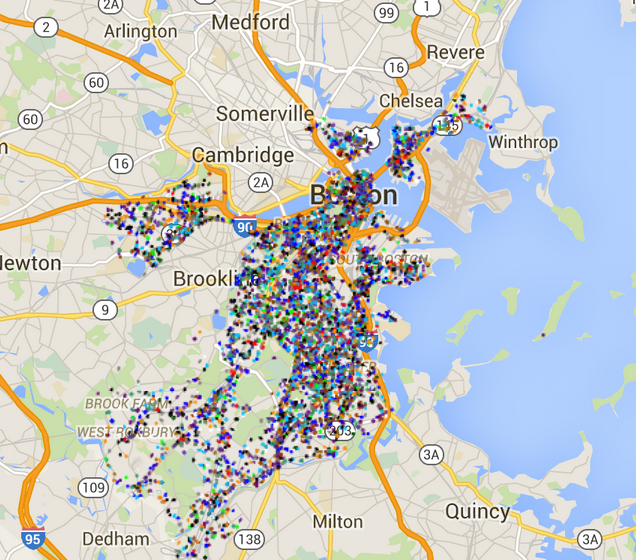
\includegraphics[width=\columnwidth]{fig1.png}
        % Create a subtitle for the figure.
        %\caption{Overall crime distribution across Boston shows concentrated crime data.}
        % Define the label of the figure. It's good to use 'fig:title', so you know that the label belongs to a figure.
        %\label{fig:tf_plot}
        %\end{center}
    %\end{figure}

\section{Results}
    As discussed before, the elementary results give a basic idea about different types of crime in the city and their distribution. For example, after plotting the clusters, we could point out which area has which type of crime as prominent activity. We can also see which areas show troubles only on weekends or only late at night. This analysis itself gives residents a slightly better picture of which areas to avoid at what times and hopefully will help law enforcers to look after these hotspots.

   In Figure 1, where there are less dots we can most probably say that these areas are the safest areas in Boston. Figure 2 shows one of the clusters and crime statistics along with timestamps. Here, we can see the areas that experienced only $Assault$ crimes and only on weekdays. Similarly, we plotted a few more clusters and Figure 3 shows the areas that experienced crimes only on a weekend and during a particular time (5 a.m to 9 a.m) .

\section{Conclusion}
    So far the we have completed collecting required data and parsed it to extract required information for Boston. The primary analysis and results are encouraging enough to pursue classification techniques to get more insight on most likely next crime. We would also like to believe our future work will reach the levels of $Minority\ Report(2002)$[7] which is where we got this idea from.

% Now we need a bibliography:
\begin{thebibliography}{5}

    %Each item starts with a \bibitem{reference} command and the details thereafter.
    \bibitem{1} % Transaction paper
    CRIME PREDICTION BASED ON CRIME TYPES AND USING SPATIAL AND  TEMPORAL CRIMINAL HOTSPOTS Tahani Almanie, Rsha Mirza and Elizabeth Lor Department of Computer Science, University of Colorado, Boulder, USA.

    \bibitem{2} 
    Crimereports.com, 2015. [Online]. Available: https://www.crimereports.com. [Accessed: 20- May-2015].
    \bibitem{3} 
    `Crime — Datasets - US City Open Data Census', Us-city.census.okfn.org, 2015. [Online]. Available: http://us-city.census.okfn.org/dataset/crime-stats. [Accessed: 20- May- 2015].
    \bibitem{4}
    Regression techniques reference. 
    \url{http://scikit-learn.org/stable/auto_examples/linear_model/plot_ols.html}
    \bibitem{5}
    GMPlot reference.
    \url{https://pypi.python.org/pypi/gmplot/1.0.5}
    
    \bibitem{6}
    GitHub code repository.
    \url{https://github.com/sahilsd/591-crime-project}
    \bibitem{5}
    Minority Report (2002)
    \url{http://www.imdb.com/title/tt0181689/}

\end{thebibliography}

% Your document ends here!
\end{document}
